\documentclass[12pt]{article}
\usepackage[left=1cm, right=1cm, top=2cm,bottom=1.5cm]{geometry} 

\usepackage[parfill]{parskip}
\usepackage[utf8]{inputenc}
\usepackage[T2A]{fontenc}
\usepackage[russian]{babel}
\usepackage{enumitem}
\usepackage[normalem]{ulem}
\usepackage{amsfonts, amsmath, amsthm, amssymb, mathtools}
\usepackage{tabularx}
\usepackage{hhline}

\usepackage{accents}
\usepackage{fancyhdr}
\pagestyle{fancy}
\renewcommand{\headrulewidth}{1.5pt}
\renewcommand{\footrulewidth}{1pt}

\usepackage{graphicx}
\usepackage[figurename=Рис.]{caption}
\usepackage{subcaption}
\usepackage{float}

%%Наименование папки откуда забирать изображения
\graphicspath{ {./images/} }

%%Изменение формата для ввода доказательства
\renewcommand{\proofname}{$\square$  \nopunct}
\renewcommand\qedsymbol{$\blacksquare$}

%%Изменение отступа на таблицах
\addto\captionsrussian{%
	\renewcommand{\proofname}{$\square$ \nopunct}%
}
%% Римские цифры
\newcommand{\RN}[1]{%
	\textup{\uppercase\expandafter{\romannumeral#1}}%
}

%% Для удобства записи
\newcommand{\MR}{\mathbb{R}}
\newcommand{\MQ}{\mathbb{Q}}
\newcommand{\MI}{\mathrm{I}}
\newcommand{\MJ}{\mathrm{J}}
\newcommand{\MH}{\mathrm{H}}
\newcommand{\MT}{\mathrm{T}}
\newcommand{\MU}{\mathcal{U}}
\newcommand{\MV}{\mathcal{V}}
\newcommand{\VN}{\varnothing}
\newcommand{\VE}{\varepsilon}

\theoremstyle{definition}
\newtheorem{defn}{Опр:}
\newtheorem{rem}{Rm:}
\newtheorem{prop}{Утв.}
\newtheorem{exrc}{Упр.}
\newtheorem{lemma}{Лемма}
\newtheorem{theorem}{Теорема}
\newtheorem{corollary}{Следствие}

\newenvironment{cusdefn}[1]
{\renewcommand\thedefn{#1}\defn}
{\enddefn}

\DeclareRobustCommand{\divby}{%
	\mathrel{\text{\vbox{\baselineskip.65ex\lineskiplimit0pt\hbox{.}\hbox{.}\hbox{.}}}}%
}
%Короткий минус
\DeclareMathSymbol{\SMN}{\mathbin}{AMSa}{"39}
%Длинная шапка
\newcommand{\overbar}[1]{\mkern 1.5mu\overline{\mkern-1.5mu#1\mkern-1.5mu}\mkern 1.5mu}
%Функция знака
\DeclareMathOperator{\sgn}{sgn}

%Обозначение константы
\DeclareMathOperator{\const}{\text{const}}

%Интеграл в большом формате
\DeclareMathOperator{\dint}{\displaystyle\int}

\newcommand{\smallerrel}[1]{\mathrel{\mathpalette\smallerrelaux{#1}}}
\newcommand{\smallerrelaux}[2]{\raisebox{.1ex}{\scalebox{.75}{$#1#2$}}}

\newcommand{\smallin}{\smallerrel{\in}}
\newcommand{\smallnotin}{\smallerrel{\notin}}

\newcommand*{\medcap}{\mathbin{\scalebox{1.25}{\ensuremath{\cap}}}}%
\newcommand*{\medcup}{\mathbin{\scalebox{1.25}{\ensuremath{\cup}}}}%

%Скалярное произведение
\DeclarePairedDelimiterX{\inner}[2]{\langle}{\rangle}{#1, #2}

%Подпись символов снизу
\newcommand{\ubar}[1]{\underaccent{\bar}{#1}}

\begin{document}
\lhead{Математический анализ - \RN{2}}
\chead{Шапошников С.В.}
\rhead{Лекция - 4}

\section*{Сходимость в метрических пространствах}
Пусть $(X, \rho)$ - метрическое пространство.
\begin{defn}
	Последовательность $\{x_n\}$ сходится к $x\colon x_n \to x$, если $\rho(x_n,x) \to 0$.
\end{defn}

\begin{prop}
	Предел определен единственным образом, то есть $x_n \to x$ и $x_n \to y \Rightarrow x = y$.
\end{prop}
\begin{proof}
	$\rho(x,y) \leq \rho(x,x_n) + \rho(x_n, y) \xrightarrow[n \to \infty]{} 0  \Rightarrow 0 \leq \rho(x,y) \leq 0 \Rightarrow \rho(x,y) = 0 \Rightarrow x = y$.
\end{proof}

\begin{prop}
	Если последовательность сходится, то она ограниченна, то есть лежит в некотором шаре.
\end{prop}
\begin{proof}
	$x_n \to x \Leftrightarrow \rho(x_n,x) \to 0 \Rightarrow \exists \, N \colon \forall n > N, \, \rho(x_n,x) < 1$. Возьмем 
	$$R = \max\{1, \rho(x_1, x),\rho(x_2,x), \dotsc ,\rho(x_N, x) \}$$
	Ясно, что $\forall x_n, \, x_n \in \overline{B}(x,R)$, то есть последовательность ограниченна.
\end{proof}

\begin{lemma}
	$|\rho(x,u) - \rho(x,v)| \leq \rho(u,v)$.
\end{lemma}
\begin{proof}
	$$\rho(x,u) - \rho(x,v) \leq \rho(u,v) \Leftrightarrow \rho(x,u) \leq \rho(x,v) + \rho(v,u)$$
	верно по неравенству треугольника.
	$$\rho(x,v) - \rho(x,u) \leq \rho(u,v) \Leftrightarrow \rho(x,v) \leq \rho(x,u) + \rho(u,v)$$
	верно по неравенству треугольника.
	
	Тогда $$-\rho(u,v) \leq \rho(x,u) - \rho(x,v) \leq \rho(u,v) \Rightarrow |\rho(x,u) - \rho(x,v)| \leq \rho(u,v)$$
\end{proof}

\begin{prop}\textbf{(непрерывность $\rho$)} 
	Если $x_n \to x$ и $y_n \to y$, то $\rho(x_n, y_n) \to \rho(x,y)$.
\end{prop}
\begin{proof}
	Используя неравенство $|\rho(x,u) - \rho(x,v)| \leq \rho(u,v)$, рассмотрим следующую разность:
	$$
		|\rho(x_n, y_n) - \rho(x,y)| = |\rho(x_n, y_n) - \rho(x_n,y) + \rho(x_n,y) - \rho(x,y)| \leq
	$$
	$$
		\leq  |\rho(x_n, y_n) - \rho(x_n,y)| + |\rho(x_n,y) - \rho(x,y)| \leq \rho(y_n, y) + \rho(x_n,x) \xrightarrow[n \to \infty]{} 0
	$$
\end{proof}

\subsection*{Метрическое пространство $\MR^n$}

Расммотрим следующее метрическое пространство: $\MR^n, \, \rho(x,y) = \sqrt{ \displaystyle \sum\limits_{k=1}^{n}(x_k - y_k)^2}$.
\begin{lemma}
	Верно неравенство $\max\limits_{1 \leq k \leq n} |x_k| \leq \sqrt{\displaystyle \sum\limits_{k=1}^{n}x_k^2} \leq \sqrt{n} \max\limits_{1 \leq k \leq n} |x_k|$.
\end{lemma}
\textbf{Пример}: Очевидно, что $\max\{|a|,|b|\} \leq \sqrt{a^2 + b^2} \leq \sqrt{2}\max\{|a|,|b|\}$.

\begin{theorem}
	Последовательность $x^m \in \MR^n, \, x^m = (x_1^m, \dotsc x_n^m)$ сходится к $x \in \MR^n, \, x = (x_1, \dotsc, x_n)$ по метрике $\rho = \sqrt{ \displaystyle \sum\limits_{k=1}^{n}(x_k - y_k)^2} \Leftrightarrow \forall k = \overline{1,n}, \, x_k^m \to x_k$. То есть сходимость в пространстве $\MR^n$ равносильна покоординатной сходимости.
\end{theorem}
\begin{rem}
	В зависимости от контекста, мы рассматриваем элементы в $\MR^n$ как точки или вектора, показывающие эти точки. Если складываем что-то, то считаем элементы векторами, а если рассматриваем метрические пространства, то видим за этим точки.
\end{rem}
\begin{proof}\hfill
	\begin{enumerate}[label={\arabic*)}]
		\item Если $|x_k^m - x_k| \leq \rho(x^m,x) \to 0 \Rightarrow x_k^m \to x_k$, по первому неравенству из леммы;
		\item Если $\forall k, \, x_k^m \to x_k \Rightarrow \max\limits_{k}|x_k^m - x^k| \to 0 \Rightarrow$ из 2-го неравенства леммы $\rho(x^m,x) \to 0$;
	\end{enumerate}
\end{proof}

\begin{theorem}\textbf{(Больцано)}
	Из ограниченной последовательности элементов $\MR^n$ можно выбрать сходящуюся подпоследовательность.
\end{theorem}
\begin{rem}
	Если не указывается метрика $\MR^n$ в явном виде, то подразумевается Евклидова метрика.
\end{rem}
\begin{proof}
	$x^m$ - ограничена $\Rightarrow x^m \in B(x^0, R) \Rightarrow |x_k^m - x_k^0| \leq \rho(x^m,x^0) \leq R, \, \forall k = \overline{1,n} \Rightarrow x_k^m$ - ограниченная последовательность $\Rightarrow$ по теореме Больцано для одномерного случая $\exists$ сходящаяся подпоследовательность, но номера могут оказаться разными $\Rightarrow$ нужно делать выбор внутри выбранной последовательности. 
	
	\uline{Первые координаты} $x_1^m$ в последовательности $x^m \Rightarrow$ возьмем сходящуюся подпоследовательность $\Rightarrow$ среди последовательности $x^m$ возьмем те номера, по которым сходится подпоследовательность первой координаты $\Rightarrow x^{m_s}$.
	
	\uline{Вторые координаты} $x_2^{m_s}$ в подпоследовательности $x^{m_s} \Rightarrow$ выделим сходящуюся подпоследовательность, при этом сходимость по первой координате сохранится в силу того, что всякая подпоследовательность сходящейся последовательности сходится к одному и тому же пределу. 
	
	Продолжим процедуру до координаты $n$ и в результате получим некоторую подпоследовательность последовательности $x^m$, сходящуюся по каждой из координат.
	
	Случай $n=2 \Rightarrow x_1^m$ - ограничена $\Rightarrow$ по теореме Больцано $\exists$ сходящаяся подпоследовательность: $x_1^{m_s} \to a_1$. Рассмотрим последовательность $x_2^{m_s}$ - ограничена $\Rightarrow$ по теореме Больцано $\exists$ сходящаяся подпоследовательность: $x_2^{m_{s_t}} \to a_2$. Если взяли сходящуюся последовательность и в ней возьмем подпоследовательность, то она будет сходиться к тому же самому $\Rightarrow x^{m_{s_t}} = (x_1^{m_{s_t}},x_2^{m_{s_t}}) \colon  x^{m_{s_t}} \xrightarrow[]{t \to \infty} (a_1,a_2)$
\end{proof}

\newpage
\subsection*{Полные метрические пространства}

\begin{defn}
	Метрическое пространство $(X,\rho)$ называется \uwave{полным}, если в нем выполняется критерий Коши, то есть: последовательность $x_n$ - сходится $\Leftrightarrow \forall \VE > 0, \exists \, N \colon \forall n, m> N, \, \rho(x_n,x_m) < \VE$. Такие последовательности называются \uwave{фундаментальными} или \uwave{последовательностями Коши}.
\end{defn}
\begin{rem}
	Из сходимости всегда следует фундаментальность: 
	$$
	x_n \to x \Rightarrow \rho(x_n,x_m) \leq \rho (x_n,x) + \rho(x,x_m), \, \forall \VE > 0, \exists \, N \colon \forall n > N,\, \rho(x_n, x) < \VE \Rightarrow
	$$ 
	$$
	\Rightarrow \forall n,m > N \Rightarrow \rho (x_n,x) + \rho(x,x_m) < 2\VE
	$$
\end{rem}
\textbf{Пример}: $\MR, \, \rho(x,y) = |x-y|$ - полное пространство (см. первый семестр).

\textbf{Пример}: $\MQ, \, \rho(x,y) = |x-y|$ - неполное пространство (на примерe про $\sqrt{2}$ или $e$: последовательность будет сходится к числу не из этого пространства $\Rightarrow$ не будет сходиться).

\textbf{Пример}: $X\neq \VN,\, \rho(x,y) = \begin{cases} 1, & x \neq y \\ 0, & x = y \end{cases}$, это \uwave{дискретная метрика}, тогда 
$$
x_n \to x \Leftrightarrow \rho(x_n,x) \to 0, \exists \, N \colon \forall n > N, \, \rho(x_n,x) < 1 \Rightarrow \rho(x_n,x) = 0
$$
По этой метрике сходятся только те последовательности, которые начиная с некоторого номера становятся постоянными. Будет ли это пространство полным? Возьмем $\VE = \tfrac{1}{2} \Rightarrow$ фундаментальность означает следующее:
$$
\exists \, N \colon \forall n, m > N, \, \rho(x_n,x_m) < \VE \Rightarrow x_n = x_m
$$ 
в частности $\forall n > N, \, x_n = x_{N+1}$ и сходятся к $x_{N+1}$. Таким образом, это полное пространство. 

\begin{rem}
	Полнота пространства зависит не только от множества, но и от метрики пространства. Пространство $\MQ$ с дискретной метрикой будет полным пространством.
\end{rem}

\textbf{Пример}: $\MR,\, \rho(x,y) = |\arctan{x} - \arctan{y}|$. В этом случае, $x_n = n$ - фундаментальна с указанной метрикой: 
$$x_n \to +\infty \Rightarrow \arctan{x_n} \to \dfrac{\pi}{2} \Rightarrow \rho(x_n,x_m) \to 0$$
но при этом последовательность не сходится (например, зафиксировали $x$, а вместо $y$ взяли $n \Rightarrow$ получим $\arctan{x} - \tfrac{\pi}{2}$) $\Rightarrow$ нет сходимости (метрика не стремится к $0$) $\Rightarrow$ неполное пространство.

\begin{theorem}
	$\MR^n$ - полное метрическое пространство.
\end{theorem}
\begin{proof}
	Пусть $x^m$ - фундаментальная $\Rightarrow$ по лемме $|x_k^m - x_k^l| \leq \rho(x^m,x^l) \Rightarrow \forall k = \overline{1,n}, \, x_k^m$ - фундаментальна $\Rightarrow x_k^m \to a_k$. То есть каждая координата сходится к какому-то пределу. Сходимость по координатам $\Leftrightarrow$ сходимости по метрике. 
\end{proof}

\subsection*{Пополнение метрического пространства}
Можно ли из неполного пространства сделать полное? Например, каким-то образом дополнить исходное неполное пространство. 

Пусть $X \subset Y$, так что на обоих пространствах одинаковая метрика. Напрямую это обычно сделать не получается, поэтому рассмотрим $f\colon X \to Y, \, \rho_Y(f(x_1),f(x_2)) = \rho_X(x_1,x_2)$, в этом случае говорят, что сделано \uwave{изометрическое вложение}. 

Хотим, чтобы $Y$ было самым маленьким полным пространством, содержащем $X$ и тогда $\overline{X} = Y$, то есть замыкание множества $X$ совпало бы с полным пространством $Y \Rightarrow Y$ - это пополнение $X$. 

\uline{\textbf{Способ пополнения пространств}}: хотим, чтобы фундаментальные последовательности $\{x_n\}$ сходились $\Rightarrow$ вместо $X$ будем рассматривать всевозможные фундаментальные последовательности:
$$
Y = \{\text{фундаментальные последовательности} \{x_n\}\}
$$ 
Мы рассматриваем фундаментальные последовательности, поскольку так мы можем разделять последовательности, которые что-то приближают и которые должны бы сходится от всех остальных последовательностей. Когда одно и то же число можно представить разными последовательностями, то
$$
\{x_n\} \sim \{y_n\} \Leftrightarrow \rho(x_n,y_n) \to 0
$$ 
Таким образом, элементы $Y$ - это классы эквивалентности. Как ввести метрику? Например 
$$
\rho(\{x_n\},\{y_n\})= \lim\limits_{n \to \infty}\rho(x_n,y_n)
$$ 
Если бы последовательности сходились, то $\lim\limits_{n \to \infty}\rho(x_n,y_n)$ сходилось бы к расстоянию между их пределами. Можно доказать, что из фундаментальности этих последовательностей, такой предел существует, можно показать, что он не зависит от выбора представителя класса эквивалентности и удовлетворяет свойствам метрики $\Rightarrow$ появилось метрическое пространство $(Y,\rho)$. 

В этом пространстве хотим найти $X \Rightarrow x \in X \mapsto \{x_n \equiv x\}$. Можно показать, что в силу определения это изометрическое вложение. Осталось проверить:
\begin{enumerate}
	\item Получившееся пространство - полное;
	\item Любой элемент $Y$ приближается ``постоянной'' последовательностью ($\{x_n \equiv x_N\}$);
\end{enumerate}
Это как раз и означает, что $\overline{X} = Y$. Таким образом добавлено лишь то, что можно приблизить элементами из $X$.

\textbf{Пример}: Таким способом можно получить вещественные числа: Есть рациональные числа $\Rightarrow$ объявляем вещественным числом - класс эквивалентности фундаментальной последовательности.

\begin{rem}
	Описанный способ пополнения не единственный, но если были какие-то свойства на $X$ помимо метрики, то они переносятся естественным способом на $Y$.
\end{rem}

\begin{exrc}
	Проверить эту процедуру пополнения и дополнить $\MQ$ до $\MR$ (см. книгу Львовский: Математический анализ).
\end{exrc}

\newpage
\section*{Сходимость в нормированных пространствах}

\begin{defn}
	Линейное пространство $X$ (над $\MR$) называется \uwave{нормированным}, если задана функция\\ $\|\cdot\| \colon X \to [0, +\infty)$, удовлетворяющая свойствам:
	\begin{enumerate}[label={\arabic*)}]
		\item $\|x\| = 0 \Leftrightarrow x = 0$;
		\item $\|\alpha x\| = |\alpha|\cdot\|x\|$;
		\item $\|x+y\| \leq \|x\| + \|y\|$ (неравенство треугольника);
	\end{enumerate}
\end{defn}
На нормированном пространстве есть метрика $\rho (x,y) = \|x - y\|$, где $\|\cdot\|$ называется \uwave{нормой}. 

Поскольку это метрическое пространство, то на нем можно определить сходимость. Но перед этим убедимся, что нормированные пространства немного лучше, чем метрические.
\begin{prop}
	В нормированном пространстве шар $B(a,R) \supset B(b,r) \Rightarrow R > r$.
\end{prop}
\begin{proof}\hfill\\
	Пусть $b = a \Rightarrow \{\, x \mid \rho(a,x) < R \, \} \supset \{\, x \mid \rho(a,x) < r \, \}$, тогда $	\forall x \in B(a,r)$
	$$
	 \rho(a,x) = \|x-a\| < R \Rightarrow \forall x \in B(a,R) \wedge x \notin B(a,r), \, r \leq \rho(a,x) = \|x-a\| < R  \Rightarrow r < R
	$$
	
	\begin{figure}[H]
		\centering
		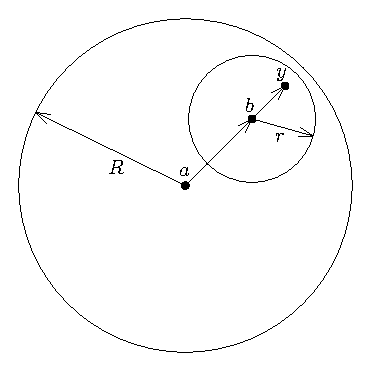
\includegraphics[width=0.35\textwidth]{4_1.eps}
		\caption{Шары в нормированном пространстве.}
		\label{4_1}
	\end{figure}
	
	Пусть $b \neq a \Rightarrow$ если $y = t\dfrac{(b-a)}{\|b-a\|} + (b-a) \in B(b,r)$, где $0 < t < r$, то получим следующее
	$$
		\bigg\| t\dfrac{b-a}{\|b-a\|} + (b-a)\bigg\| < R \Rightarrow
		\bigg\| t\dfrac{(b-a)}{\|b-a\|} + (b-a)\bigg\| = \bigg\| \bigg(1 + \dfrac{t}{\|b-a\|}\bigg)(b-a)\bigg\| =
	$$
	$$	
		=  \bigg(1 + \dfrac{t}{\|b-a\|}\bigg)\|b-a\| = t + \|b-a\| < R, \, \forall\, 0< t < r
	$$
	Устремляем $t \to r \Rightarrow t + \|b-a\| < R \to r + \|b-a\| \leq R \Rightarrow r < R$, так как $\|b-a\| >0$.
\end{proof}
\newpage
\begin{prop}
	Если в нормированном пространстве $x_n \to x, \, y_n \to y, \, \alpha_n \in \MR \colon \alpha_n \to \alpha$, то 
	\begin{enumerate}[label={(\arabic*)}]
		\item $x_n + y_n \to x + y$;
		\item $\alpha_n \cdot x_n \to \alpha \cdot x$;
	\end{enumerate}
\end{prop}
\begin{proof}Пусть $x_n \to x, \, y_n \to y, \, \alpha_n \in \MR \colon \alpha_n \to \alpha$, тогда
	\begin{enumerate}[label={(\arabic*)}]
		\item По определению: 
		$$
			\|(x+y) - (x_n + y_n)\| = \|(x-x_n) + (y - y_n)\| \leq \|x - x_n\| + \|y - y_n\| \to 0
		$$
		\item По определению: 
		$$
			\|\alpha_n x_n - \alpha x \| = \|(\alpha_n x_n - \alpha_n x) + (\alpha_n x - \alpha x)\| \leq |\alpha_n|{\cdot} \|x_n - x\| + |x| {\cdot}\|\alpha_n - \alpha\|
		$$ 
		Поскольку $\alpha_n \to \alpha \Rightarrow$ это ограниченная последовательность и $x_n \to x$, то 
		$$
			|\alpha_n|{\cdot} \|x_n - x\| +  |\alpha_n - \alpha|{\cdot}\|x\| \to |\alpha|\cdot 0 + 0 \cdot \|x\| = 0
		$$
	\end{enumerate}
\end{proof}

\begin{exrc}
	Доказать:
	\begin{enumerate}[label={\arabic*)}]
		\item $\big|\|x\| - \|y\|\big| \leq \|x-y\|$
		\begin{proof}
			Используем лемму: $|\rho(z,x) - \rho(z,y)| \leq \rho(x,y) \Rightarrow z = x + y \Rightarrow$
			$$|\rho(z,x) - \rho(z,y)| = \big|\|x + y - x\| - \|x + y - y\|\big| = \big|\|x\| - \|y\|\big| \leq \|x -y\|;$$
		\end{proof}
		\item $x_n \to x \Rightarrow \|x_n\| \to \|x\|$
		\begin{proof}
			По определению $x_n \to x \Leftrightarrow \rho(x_n,x) \to 0 \Rightarrow \|x_n - x\| \to 0 \Rightarrow$ используя утверждение выше:
			$$ 0 \leq \big|\|x_n\| - \|x\| \big| \leq \|x_n - x\| \to 0 \Rightarrow \|x_n\| \to \|x\|;
			$$
		\end{proof}
	\end{enumerate}
\end{exrc}

\subsection*{Нормы в $\MR^n$}
Пусть $x = (x_1, \dotsc, x_n) \in \MR^n$, тогда можно рассматривать следующие нормы:
\begin{enumerate}[label={(\arabic*)}]
	\item $\|x\|_{l_2} = \sqrt{\displaystyle \sum\limits_{k=1}^{n}x_k^2}$ (Евклидова норма);
	\item $\|x\|_{l_\infty} = \max\limits_{1 \leq k \leq n} |x_k|$;
	\item $\|x\|_{l_1} = \displaystyle \sum\limits_{k=1}^{n}|x_k|$
\end{enumerate}
\begin{theorem}
	Если $\|\cdot\|_1$ и $\|\cdot\|_2$ - произвольные нормы на $\MR^n$, то существуют числа $c_1, c_2 > 0 \colon \forall x \in \MR^n$
	$$
	c_1 \|x\|_1 \leq \|x\|_2 \leq c_2 \|x\|_1
	$$
\end{theorem}

\end{document}